%
\chapter{提案手法}
%
\section{モデル概観}
この章では,提案モデルがもつ複合特徴量生成器とニュース分類器について紹介する.
その後にこの2要素を統合して転移学習が可能な表現を学習する方法について説明する.
% 最後に,詳細なアルゴリズムフローを付加する. 
今回提案したモデルは,以下の図\ref{fig:model}の通りである.

提案モデルの目的は,画像と文章で発信された情報に対して,
正しいニュースか・フェイクニュースか・ジョークニュースかを分類するために,
必要な特徴表現を学習することであった.
提案モデルは複合特徴量生成器とニュース分類器の大きく2部分に分けることができた.
まず複合特徴量生成器は,今回扱う情報が文章と画像を含むため,
各メディアに対して特徴化する生成器があった.
その後それぞれの特徴を1つに連結し,複合特徴を形成した.
複合特徴はニュース分類器に送られ,最終的には3カテゴリのどれに該当するかが判断された.
% 
\begin{figure}[H]
    \centering
    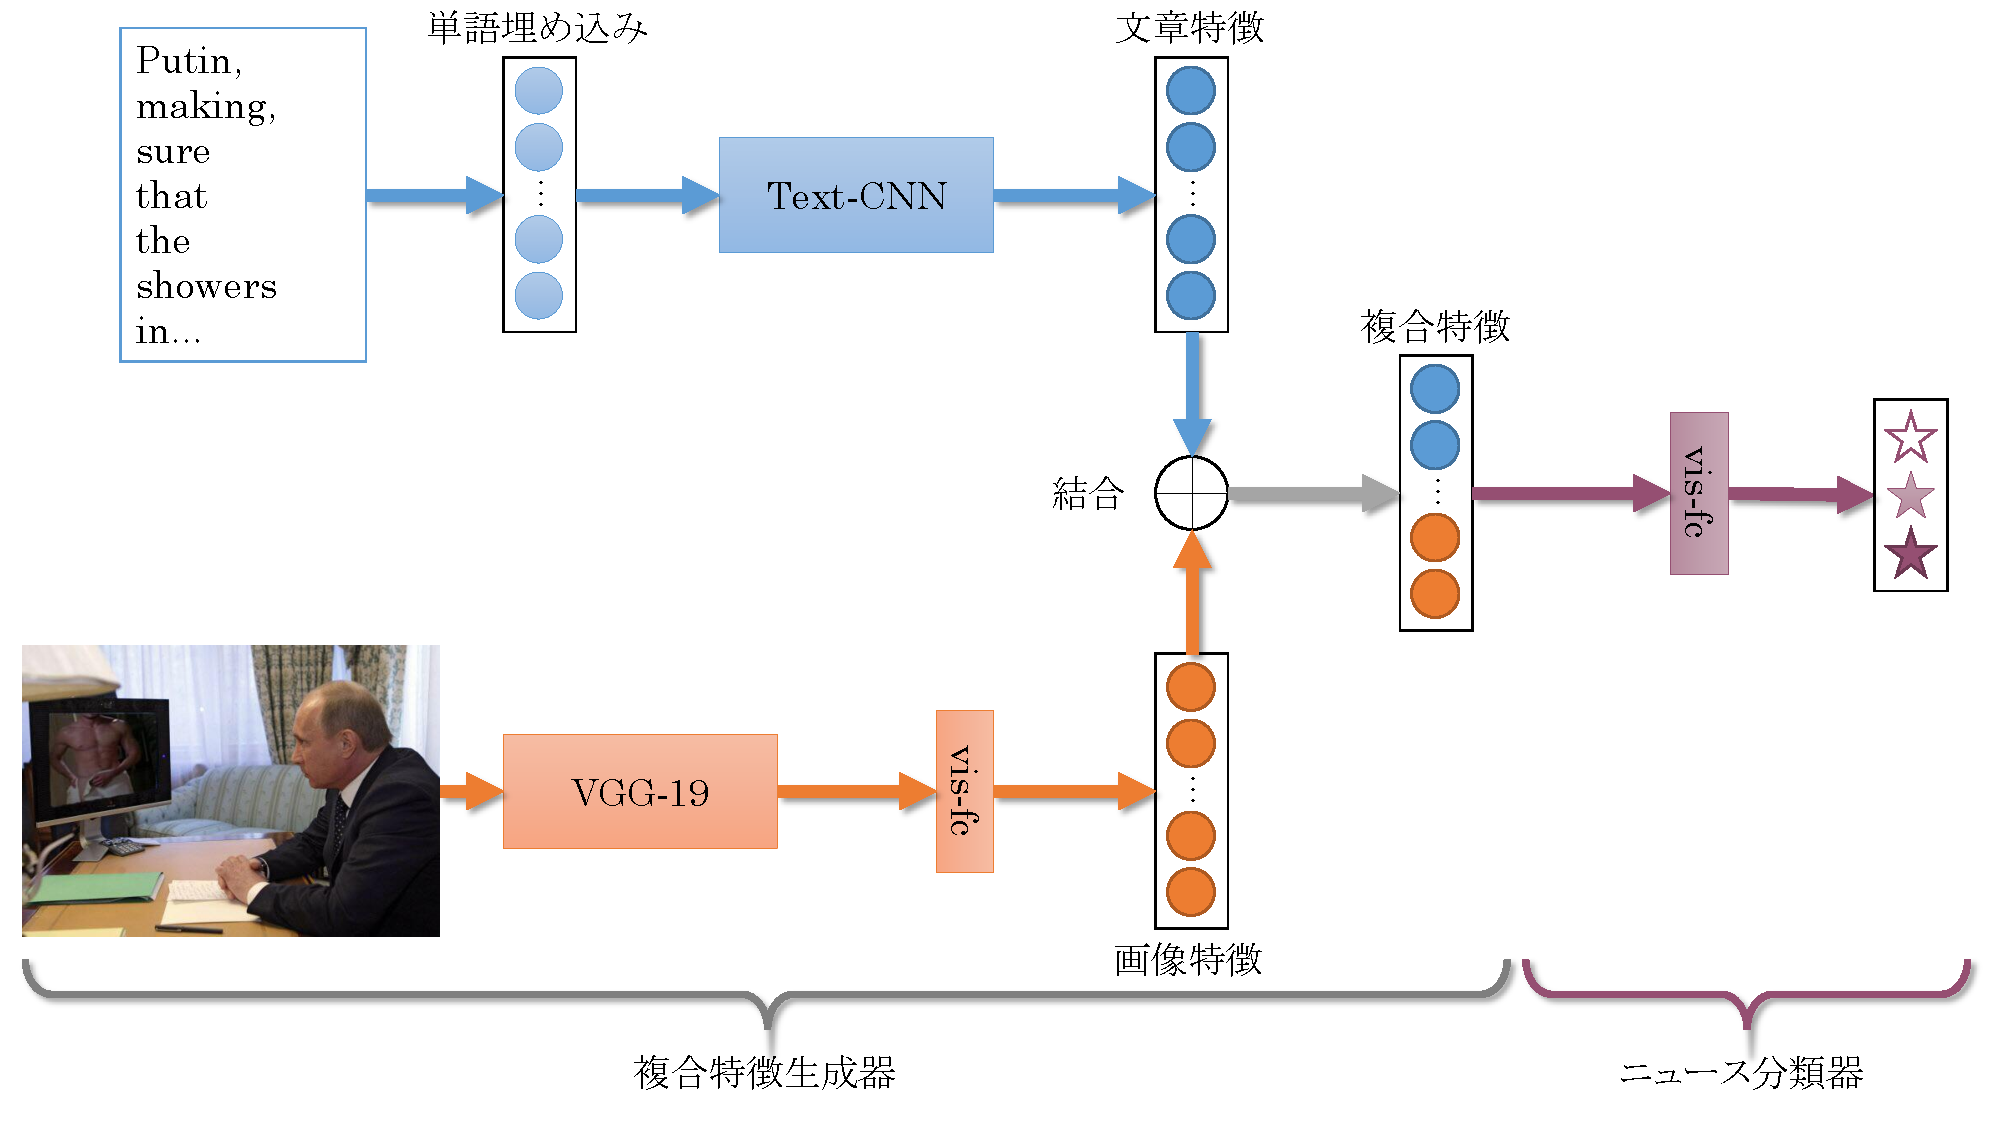
\includegraphics[width=\linewidth]{images/methodology.pdf}
    \caption{提案モデル図.青色が文章特徴量生成器,橙色が画像特徴生成器,紫色がニュース分類器であった.}
    \label{fig:model}
\end{figure}
%
\section{複合特徴生成器}
%
\subsection{文章特徴}
文章特徴は,入力に英語の投稿をスペース毎に分割した英単語の連続リストをもった.
まずは単語を単語埋め込みでベクトル化した.
その後単語の羅列から分類に有効な情報を得るために,文章特徴を生成する核としてCNN
(convolutional neural networks: 畳み込みニューラルネットワーク)を採用した.
CNNはコンピュータビジョンやテキスト分類などの多くの分野で効果的であることが示されていた
\cite{collobert2011natural,kalchbrenner2014convolutional}.
図\ref{fig:model}の通り,提案手法ではCNNの発展形であるテキストCNN(Text-CNN)\cite{kim2014convolutional}を採用した.
テキストCNNの構造は図\ref{fig:text-cnn}の通りである.
複数のウィンドウで畳み込むことで,様々な角度から特徴を抽出することを実現した.
\begin{figure}[H]
    \centering
    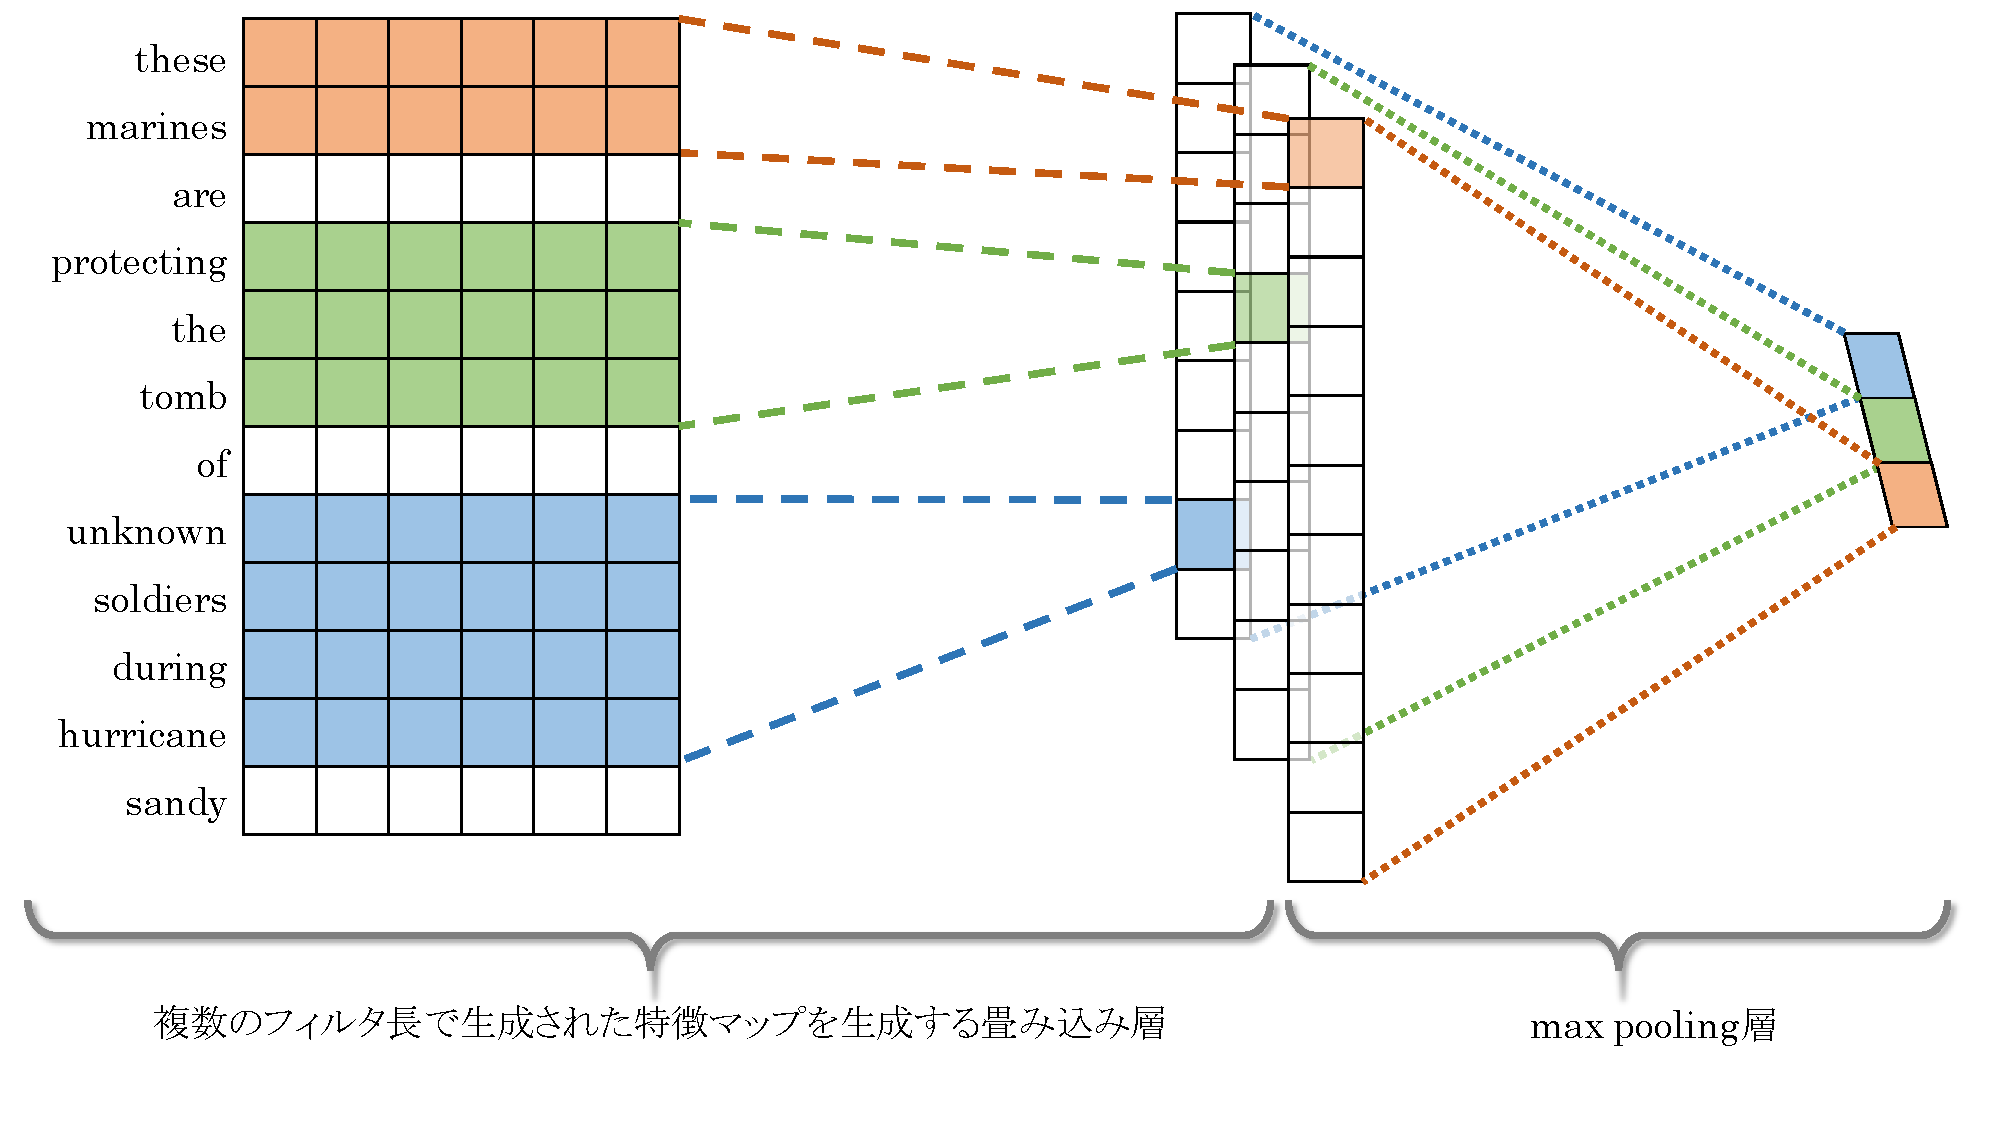
\includegraphics[width=\linewidth]{images/text-cnn.pdf}
    \caption{テキストCNNの図.Wangらの研究\cite{wang2018eann}を参考に作成.}
    \label{fig:text-cnn}
\end{figure}

具体的な手法では,EANNが採用したテキストCNNと全く同じ流れを採用した\cite{wang2018eann}.
%
\subsection{画像特徴}
画像から効率的に特徴を生成するために,当研究では事前学習済みのVGG-19\cite{simonyan2014very}を起用した.
VGG-19は畳み込み13層と全結合層3層から形成され,最終的には1000次元の特徴ベクトルが出力された.
当研究では最終の全結合層のみ改変し,文章特徴のベクトル次元数と同じ数の次元をもつベクトルを出力されるようにした.
また改変した最終全結合層以外は,過学習を防ぐために事前学習の状態を維持することにした.

こうして文章特徴・画像特徴が生成され,最終的には2つの特徴ベクトルを1つに連結したものが複合特徴となった.
%
\section{ニュース分類器}
%
複合特徴はニュース分類器にて正しいニュース・フェイクニュース・ジョークニュースとして分類された.
具体的には隠れ層を含む全結合層とsoftmaxから形成され,最終的な分類が行われた.


%図の挿入


%
%
\newpage
%
%
%
%
%
%
%
%
%
%
% 
